\section{System Architecture}

\subsection{Nodes and communication}
The following diagram refers to the architecture of our HPCS system: the functional computation and communication blocks of each of the nodes (device, edge, cloud)  and the connectivity among them.
The different implementation options for each of these nodes are listed in the following section as a set of tables with price, features, critical requirements for every element in our IoT chain.

\begin{figure}[h]
    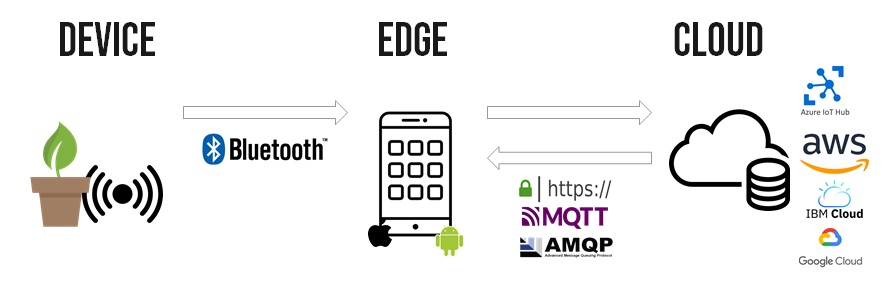
\includegraphics[width=\linewidth]{images/system-architecture.jpg}
    \caption{System architecture}
    \label{fig:System architecture}
\end{figure}

\subsection{Device hardware with sensors}
The device architecture is composed of a microcontroller (MCU board) connected to four sensors according to the following communication types: 

\begin{figure}[h]
    \centering
    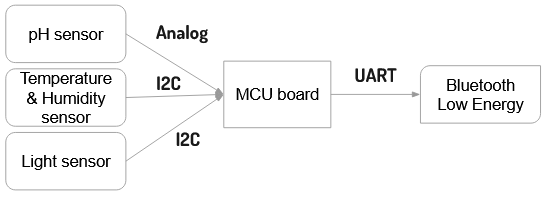
\includegraphics[width=\linewidth]{images/device-architecture.jpg}
    \caption{Device architecture}
    \label{fig:Device architecture}
\end{figure}

Digital sensors are capable of monitoring operating conditions within a specified range. Analog sensors are more advanced and provide continuous visibility of current conditions through accurate measurements. To meet the precise measurement requirements of our system, we will use analog sensors.
Since the USB interface is used when the Bluetooth module is connected as a separate dongle, we use the UART interface which is suitable for integrating a bluetooth chip into a system \cite{b6}.